\chapter{Urban Data analysis}\label{ch:uda}

\textcolor{red}{FINAL - TO BE READ ONE LAST TIME - ADD CONCLUSION IF HAVE TIME}

In this chapter, we introduce the state-of-the-art on urban data analysis.
We justify the choice of urban data as a privileged form of spatio-temporal data useful for a PhD thesis like this one, due to its variety and availability.
Section~\ref{sec:uda-motivation} presents relevance and motivations of the urban data analysis with an overview of the most important research works in the field.
In Section~\ref{sec:uda-analysis}, we present the different dimensions of urban data analysis, related to content, time and space (and a combination of them).
Section~\ref{sec:uda-solution} presents an overview of relevant examples of implementations of RDF stream processing concepts at work on urban data.
RSP represents a suitable solution because of the variety and velocity of the data sources and because of the need to fuse static (slowly evolving) and streaming data.
The first examples (see Section~\ref{sec:uda-starcity} and Section~\ref{sec:uda-trafficlark}) exploit data from different urban sources and the capability of RSP to abstract the real nature of the data through OBDA (see Section~\ref{sec:obdi-obda}) that helps the machinery and the final user to extract insights from data.
The two examples in Section \ref{sec:uda-bottari} and in Section \ref{sec:uda-london}, mainly exploit data from Twitter. The data from social network has an intrinsic graph nature and was extracted using the official APIs that return the data in JSON format. Therefore, it is easy to transform it in JSON-LD\footnote{\url{https://json-ld.org/}}, a format compatible with Semantic Web technologies. The usage of an RDF stream processor in this scenario is natural.

\section{Relevance and Motivation}\label{sec:uda-motivation}
The relevance of urban computing, or urban informatics, has been recognized since long. A recent survey on urban sensing \cite{DBLP:journals/csur/CalabreseFB14} clearly shows the value of mobile phone data to get insights of urban dynamics and human activities. 

Studies like Gonzalez et al.~\cite{gonzalez2008understanding} focus on using the mobile phones data, namely the call data records (CDRs), to track individual motion patterns characterizing each individual using a time-independent travel distance parameter and a significant probability to return to a few highly frequented locations. Candia et al.~\cite{candia2008uncovering} investigate patterns of calling activity at the individual level and show that the inter-event time of consecutive calls is heavy-tailed. 
In recent years, the analysis of telco data in such an individual way rises serious privacy issues.

However, it is also possible to use telco data in privacy preserving way.
A common applications is to use CDRs to estimate the density of crowds and vehicles in different urban regions~\cite{mcardleanalyzing,caceres2012exploring}. Another example involves the detection of people habits. Ratti et al.~\cite{ratti2006mobile} present the Mobile Landscape project, one of the first urban analysis based on the geographical mapping of cell phone usage at different times of the day in the metropolitan area of Milan. Becker et al.~\cite{becker2011tale} capture key mobility patterns within Morristown, NJ, by identifying users' home and work locations from CDRs. This information is particularly useful for urban managers and authorities that are responsible for efficient public transportation systems. Also De Nadai et al.~\cite{de2016death} test the four Jacobs conditions\footnote{The four conditions exposed by Jane Jacobs in~\cite{jacobs1961death}: mixed land uses, small blocks, buildings diversity in terms of age and form and sufficient dense concentration of people and buildings} that promote life in cities by using CDRs. Wesolowski et al.~\cite{wesolowski2013impact} combine CDRs with other cellphone-related logs (e.g., tower pings, cellular handovers) in order to compare human mobility patterns derived from CDRs.

Although mobile phones data is a priceless source to gather underlying patterns of cities and their citizens, they have got some limitations since they cannot reveal any information about people interests and thoughts. Social media data represents an opportunity to access information at individual level without violating privacy. This data is, indeed, made public by the user through a self determination process.
Social media streams are a powerful mean to explore people opinions and preferences with regard to specific venues and events.
For instance, Hristova et al.~\cite{hristova2016if} analyze temporal, spatial, and microeconomic patterns of sport game attendees to understand the users' dynamics, while Lee et al.~\cite{lee2016not} and Cho et al.~\cite{cho2011friendship} use social networks and cell phone location data, to identify humans' mobility patterns. Psyllidis et al.~\cite{psyllidis2015platform} concentrate their effort on wide range of urban data and create a web-based platform to support city planning and decision-making. In particular, Singh et al. \cite{singh2010social} introduce the concept of \textit{social pixel} that aggregates social interests of users about particular themes and locations. 
This notion plays a key role during the development of our conceptual model presented in Chapter~\ref{ch:conceptual}.

Moreover, urban data from different sources (e.g., CDRs, social data, IoT, etc.) can be merged to reveal even more interesting insights on city dynamics and urban monitoring. 
The platform built by Calabrese et al.~\cite{calabrese2011real} combines the users' mobile phones' data with the real-time location of buses and taxis to model the car traffic in Rome. Botta et al.~\cite{botta2015quantifying} try to quantify the dimension of the crowd by exploiting a combination of CDR and social media data.
Quercia and his colleagues \cite{quercia2011mobile} use CDRs to study human mobility related to special planned events in Boston. Calabrese et al. \cite{calabrese2010geography} show that there is a high correlation between the kind of event, e.g., sport, theater, music, family events, and the home location area of its attendees. Quercia et al. \cite{quercia2010recommending} build a recommendation system for social events and find out that the most effective algorithm recommends those events that are popular among local residents.

Sentiment analysis covers a wide range of applications in cities. Authors in \cite{ahmed2016smart} propose a city sensing architecture from Twitter data to monitor user opinions about events and topics. Hawelka et al. \cite{hawelka2014geo} and Calabrese et al. \cite{calabrese2010human} analyze geo-located Twitter messages and geographical preferences in order to predict global patterns of human mobility.

One of the features of interest for policy makers and cities managers~\cite{habitat2016urbanization} is the extremely diversified composition of the language mix, or multilingualism. This interest is motivated by the increasing immigration flows towards cities~\cite{sanderson2015world}, which result in rapidly changing population density~\cite{deville2014dynamic}. Multilingualism has also a broad scope in academia. In particular, different papers approach the issue of multilingualism from a historical perspective. Leimgruber in \cite{leimgruber2013management}, for example, analyses the city of Singapore, Garcia et al.~\cite{garcia2001multilingual} the city of New York, Extra et al.~\cite{extra2004urban} develop a cross-linguistic perspective on Gothenburg, Hamburg, The Hague, Brussels, Lyon and Madrid.
Moreover, Tasse et al.~\cite{tasse2016generating}, Arnaboldi et al.~\cite{arnaboldi2016studying} and Bokanyi et al.~\cite{bokanyi2015race} characterize cities and their neighborhoods from different aspects namely safety, culture and demographics through social media networks. Quaggiotto et al. \cite{quaggiotto2010new} present a tool called City Murmur with the aim at showing how different media describe the urban space through the attention that is payed on each street of a city. It wants to build a time-based narration, an historical archive of media coverage of the urban space which is able to reveal some hidden dynamics useful for city policy support, critical media analysis, and sociocultural research.

The interest around the exploitation  of urban data are growing, however the joined use of multiple data sources has not yet been fully explored.
In the next sections, using technologies meant to tame velocity and variety simultaneously (see Section~\ref{sec:rsp-mid}), we present different use cases of urban streaming data analysis.

\section{Urban Data Analysis Dimensions} \label{sec:uda-analysis}
The urban data analysis can be developed on three different dimensions: \textbf{space}, \textbf{time}, and \textbf{content}. In this section, we summarize the characteristic of each analysis dimension. See Section~\ref{sec:conc-fr-2-analysis} for more information about how our conceptual model (proposed in Chapter~\ref{ch:conceptual}) enables the described analysis dimensions

\subsection{Content Analysis}
The content can be associated to an event and thus indirectly to the time and space of the happening, and carries information that represents a measure of intensity of a tracked event.
During a content based analysis of urban data, a stakeholder can be interested about the contextual and behavioral knowledge about what and how users share about an event. 

The content analysis can be approached in two different ways: (i) using the \textit{Original} content, or (ii) creating \textit{Augmented} content.
In the former approach, the original content is analyzed as is and used for profiling social media users who are engaged in events. In the latter one, the augmented content can be created by using concept and feature extraction techniques from the original content for the purpose of more complex analysis about the events and their attendees.

The augmented content could consist of different media types including text, image, video, etc. that also contain low-level information about events like locations, time tables, related social users and so forth. From such content, \textbf{low-level features} such as color schema for images or n-gram distribution for text, can be extracted. For instance, a system can use the main color schema in photos related to an event to verify the correctness of the estimated location of that event. Furthermore, \textbf{high-level features} like number of people and their demographics in a photo, list of existing concepts that are represented in a photo or a video (using deep learning techniques) or semantic entities from text using ontology-based matching, can be extracted.

\subsection{Spatial Analysis}
Another dimension of interest in city analyses is space. Therefore, a urban analytics system must focus on analyzing events, people presence and flow, content and opinion sharing, or any other type of phenomena (like electrical consumption, traffic, economical value) with respect to the spatial distribution and spreading, also considering its dynamics in time. 
The spatial dimension is more complex to deal with than one can expect. Indeed, in smartcity context, the data sources may vary a lot: some information may refer to specific geographical points (geo-coordinates), some others may refer to venues or locations (restaurants or other public or private spaces), while others can provide information referring  to broad areas, possibly with different size and shape. Any analysis considering two or more different data sources need to keep this into account.

Interesting types of relevant analysis categories can be:
\begin{enumerate}
\item \textit{Dispersion}: studying the spatial distribution of locations of events, in particular with respect to the deviation from purely random configuration. This can be achieved with measures such as the Gini coefficient~\cite{yitzhaki1983extension}.
\item \textit{Distance and relation to places}: studying the spatial relation of events with respect to a set of given locations (e.g., stores or venues for specific happenings such as fashion shows, see Section~\ref{sec:cs-mfw}). This is covered by simple measures such as the average Euclidean distance between event and location, or the average Manhattan distance over an artificial grid of cells or travel distance over the road network.
\item \textit{Correlation}: studying the relevant correlations between different signals along the space dimension (e.g, within and across administrative boundaries). 
\item \textit{Prediction}: defining predictive analytics along the space dimension, by analyzing historic series of data and comparing it with the most fresh information from given geographical area.
\end{enumerate}

\subsection{Temporal Analysis}
Temporal analysis focuses on the study of the evolution and spreading of signals over time (e.g., measuring how fast information about an event propagates). 
The goals of temporal analysis can be diverse. We identify the following types of relevant analysis categories:
\begin{enumerate}
\item \textit{Description}: consisting in defining the signal as a time series in order to have a view of the evolution of information flows over time.
\item \textit{Correlation}: studying the temporal correlation between different time series and infer common behaviors and dynamics.
\item \textit{Prediction}: allowing generating temporal prediction over observed or correlated phenomena.
\item \textit{Anomaly detection}: identifying discrepancies between expected temporal behaviors and actual happenings.
\item \textit{Causality}: determining possible causality relations between different events.
\end{enumerate}

\subsection{Combined Time and Space Analysis}
Given the basic space and time analysis aspects described above, the subsequent level of interest is the combined analysis along both directions. A system can combine techniques described in the previous sections for running analysis across time and space. 

Furthermore, one can define time series of values that are aggregated or calculated on geographical basis. For instance, a system can define the time series of the values of the Gini Index or of the average distance of events from a set of given venues, and then analyze them along the temporal axis. 

\section{Existing Semantic Web-Based Solutions}\label{sec:uda-solution}

The next sections present four different solutions for urban data analysis based on Semantic Web technologies.
Section~\ref{sec:uda-starcity} and Section~\ref{sec:uda-trafficlark} present respectively STAR-CITY and Traffic LarKC, two works that face the problem, from architectural point of view. Both of the presented solutions perform \textit{spatial} and \textit{temporal} analysis on the collected data to offer the best route to the user based on weather, traffic and other multiple external sources.
In Section~\ref{sec:uda-london} we propose an overview of the infrastructure we created for monitoring crowds movement during the 2012 Olympic Games in London. The solution exploits data from social network and perform \textit{content}, \textit{spatial} and \textit{temporal} analysis to spot emerging pattern and mobility dynamics and enables the creation of complex data visualizations.
Finally, Section~\ref{sec:uda-bottari} presents BOTTARI, a mobile application that performs \textit{content}, \textit{spatial} and \textit{temporal} analysis on social network and urban data to recommend restaurants to the user.

\subsection{Monitoring Traffic Using Semantic and Stream Technologies} \label{sec:uda-starcity}
In recent years, public administrations and governments are embracing Open Data in the attempt to made available information to increase transparency and improve accountability of public services. Many cities are offering data regarding transportation, environment, energy and planning. Web sources offer an abundance of information (e.g., ~weather information, bike sharing usage, etc.) and non-public data can also be accessed (e.g., current location and state of public transportation, CCTV images, etc.).
Lecue et al.\cite{DBLP:journals/ws/LecueTHTBST14} proposes Semantic Traffic Analytics and Reasoning for CITY (STAR-CITY), a solution designed to ease the integration of data characterized by variety (structured and unstructured), velocity (static and real time streaming data) and volume (large amount of historical data).

\begin{figure}[t]
	\centering
	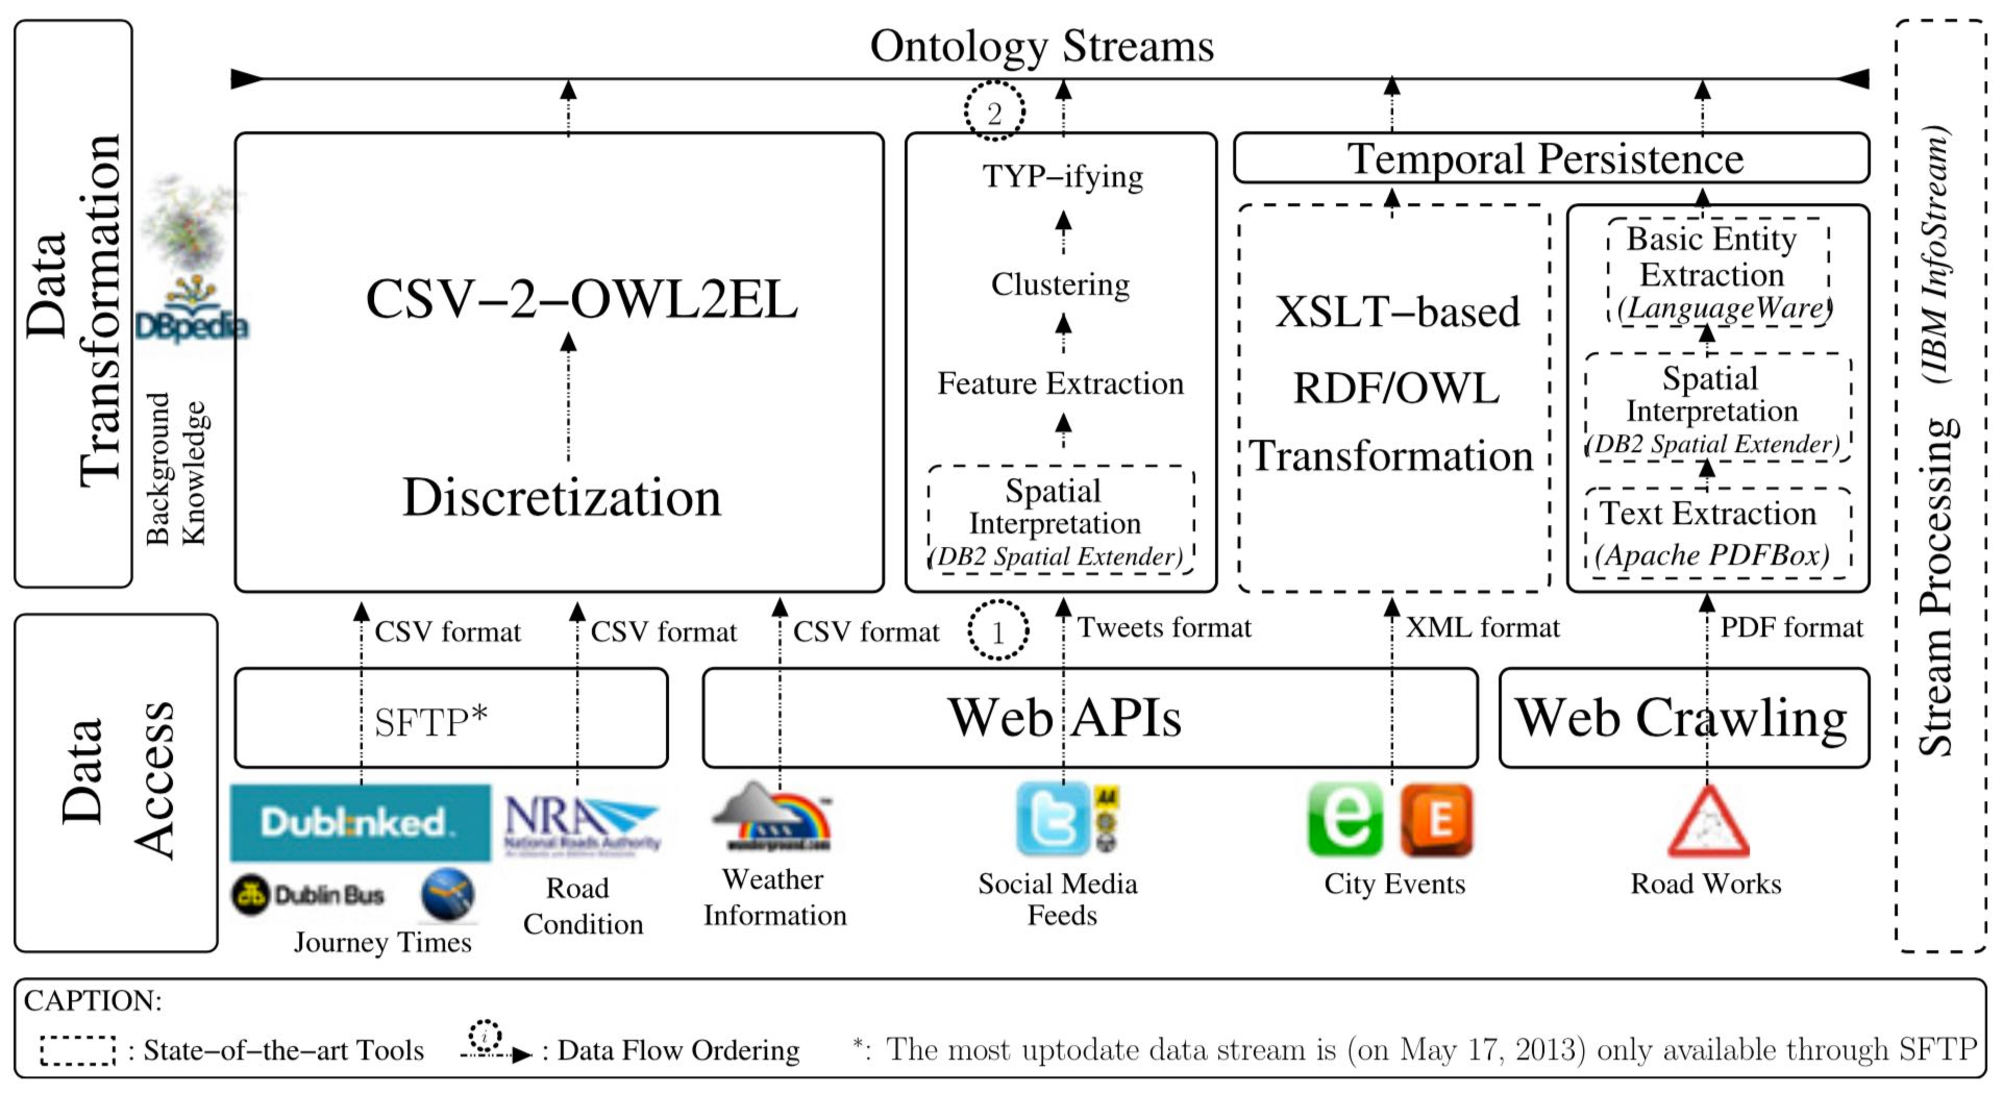
\includegraphics[width=0.75\textwidth]{img/starcity}.
    \caption{The STAR-CITY semantic stream enrichment (source~\cite{DBLP:journals/ws/LecueTHTBST14}).}
    \label{fig:star-city}
\end{figure}

STAR-CITY exploits the W3C Semantic Web stack to represent the semantics of information and to elaborate the outcomes through a combination of reasoning techniques (Figure~\ref{fig:star-city} shows STAR-CITY semantic stream enrichment architecture). The solution was mainly designed to perform \textit{spatial} and \textit{temporal} analysis on heterogeneous data, on order to provide insights on historical and real-time traffic conditions.
The traffic scenario was chosen because most of the industrial countries are suffering of traffic congestion and transportation issues that can reduce the health of citizenship and can interfere with the passage of emergency vehicles.
The system was successfully tested in various scenario involving different cities (Dublin, Bologna, Miami and Rio).

\subsection{Semantic Traffic-Aware Routing} \label{sec:uda-trafficlark}
In the late 2000s, the increasing usage of mobile technologies to get directions and information about the surrounding presented various challenges. Those challenges were only partially solved by the existing research: operation research solved the routing problem, machine learning addressed traffic forecasting, and semantic technologies managed data integration and information retrieval. Therefore, the research of location-based comprehensive solution was still an open problem.

\begin{figure}[t]
	\centering
	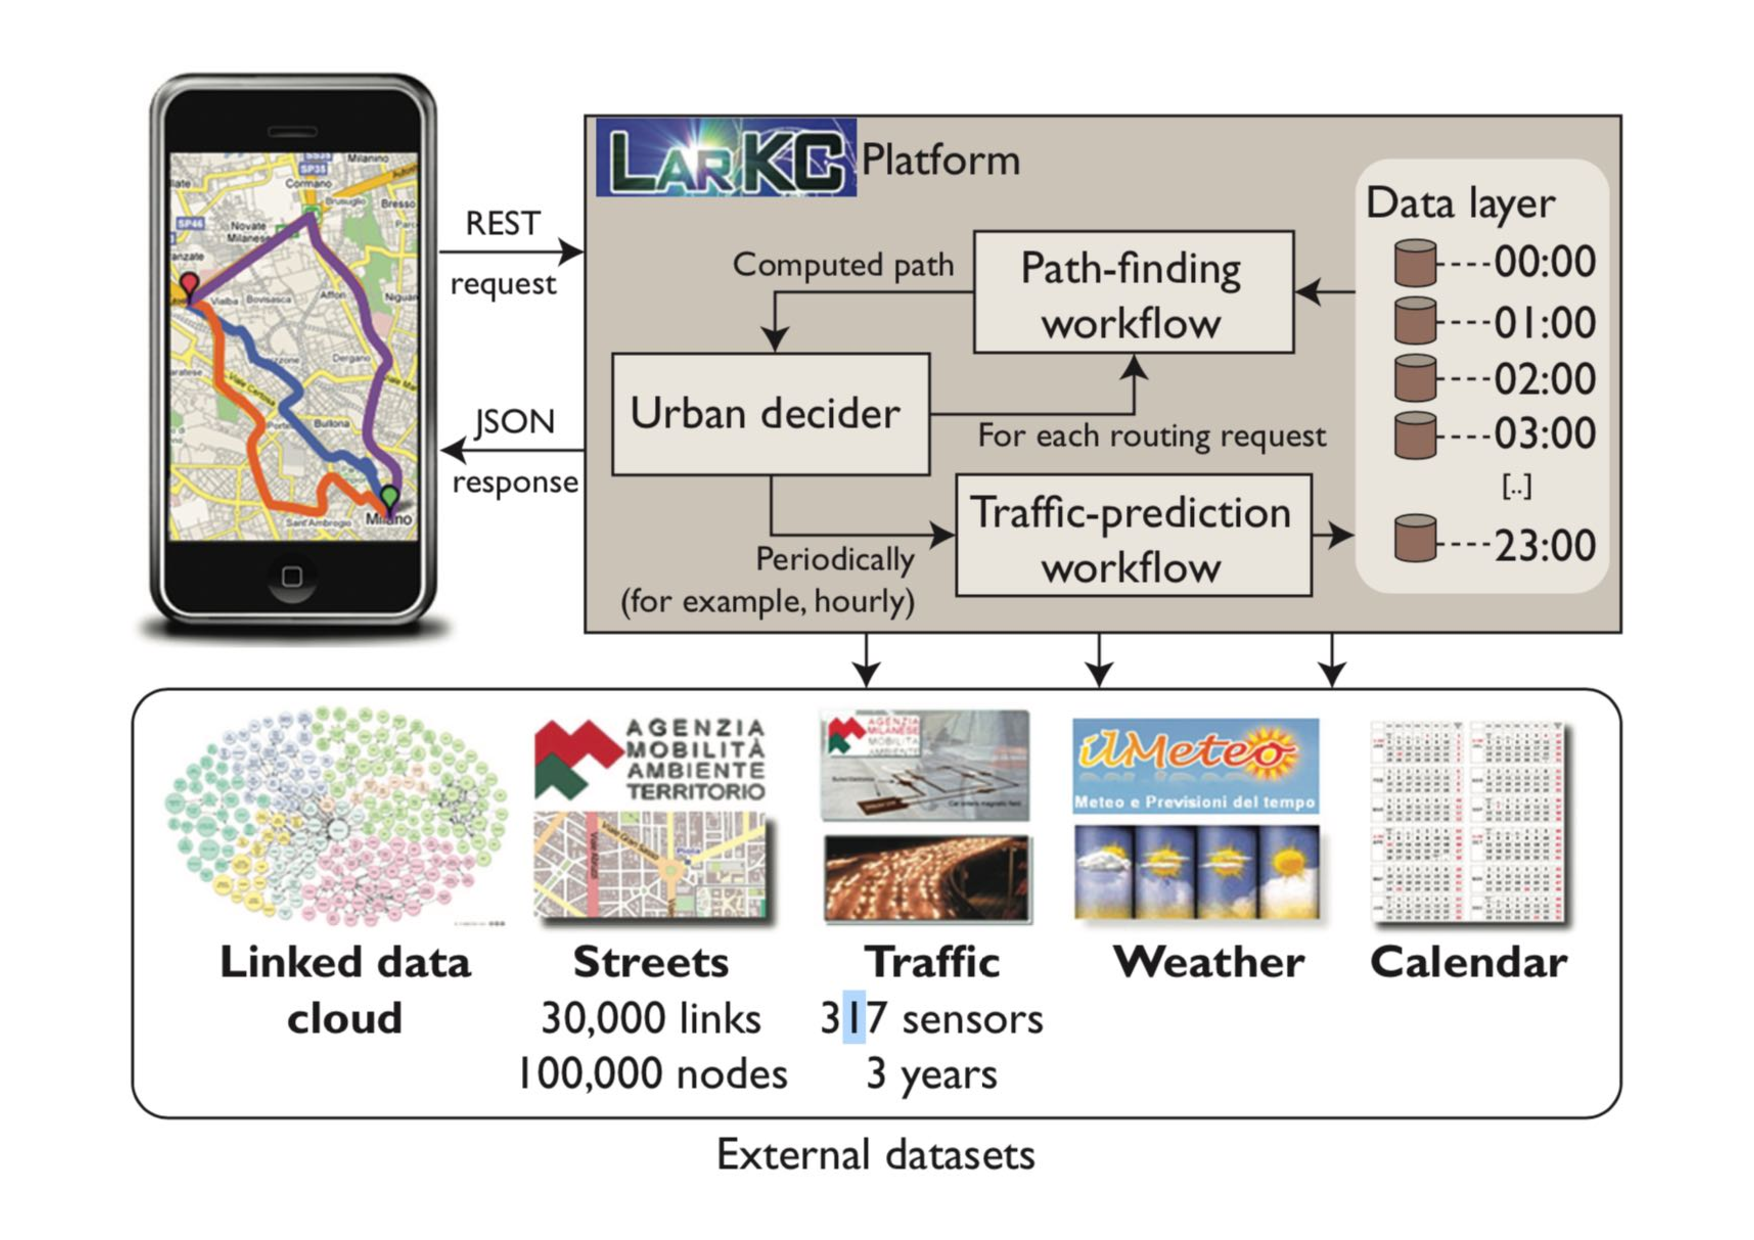
\includegraphics[width=0.75\textwidth]{img/traffic-lark.pdf}.
    \caption{The Traffic LarKC workflows and external datasets (source~\cite{DBLP:journals/internet/ValleCDGST11})}
    \label{fig:traffic-lark}
\end{figure}

Traffic LarKC~\cite{DBLP:journals/internet/ValleCDGST11} is a fist attempt to build a comprehensive system able to tame of those challenges simultaneously.
It offers a mix of conceptual query answering, machine learning, and operations research.
It can answer questions like "What Asian restaurant can I reach in less than 15 minutes if I get into my car at 6 p.m.?". 

Figure \ref{fig:traffic-lark} depicts the Traffic LarKC workflows. The service exploits the LarkC platform\cite{DBLP:conf/semco/FenselHABCVFHKLSTWWZ08} to offer a comprehensive solution to periodically perform \textit{spatial} and \textit{temporal} analysis on the data and compute the best route taking in account weather, traffic and other data from external dataset.

\subsection{Monitoring Crowd Movement During London 2012 Olympics Games} \label{sec:uda-london}
The work presented in this section shows how to track the movements of the crowds in big events exploiting the analysis of geo-tagged tweets.
Previous work shows that the data from social network is incomplete and inconsistent (see Section~\ref{sec:vel-var-solutions}) and the proposed system must deal with these data characteristics.

The presented system exploits the C-SPARQL Engine~\cite{DBLP:journals/ijsc/BarbieriBCVG10} within SLD (see Section \ref{sec:sld}) framework in order to perform \textit{content}, \textit{spatial} and \textit{temporal} analysis on Social Media streams (i.e., Twitter). 
It models the data in a convenient format and exploits OBDA to extract the position on the interesting geo-tagged tweets. 
Being public not only the position of the tweet but also the content, the system can track the people attention and select only the tweets with content related to the event. 

\begin{figure}[t]
\centering
\subfloat[]{
	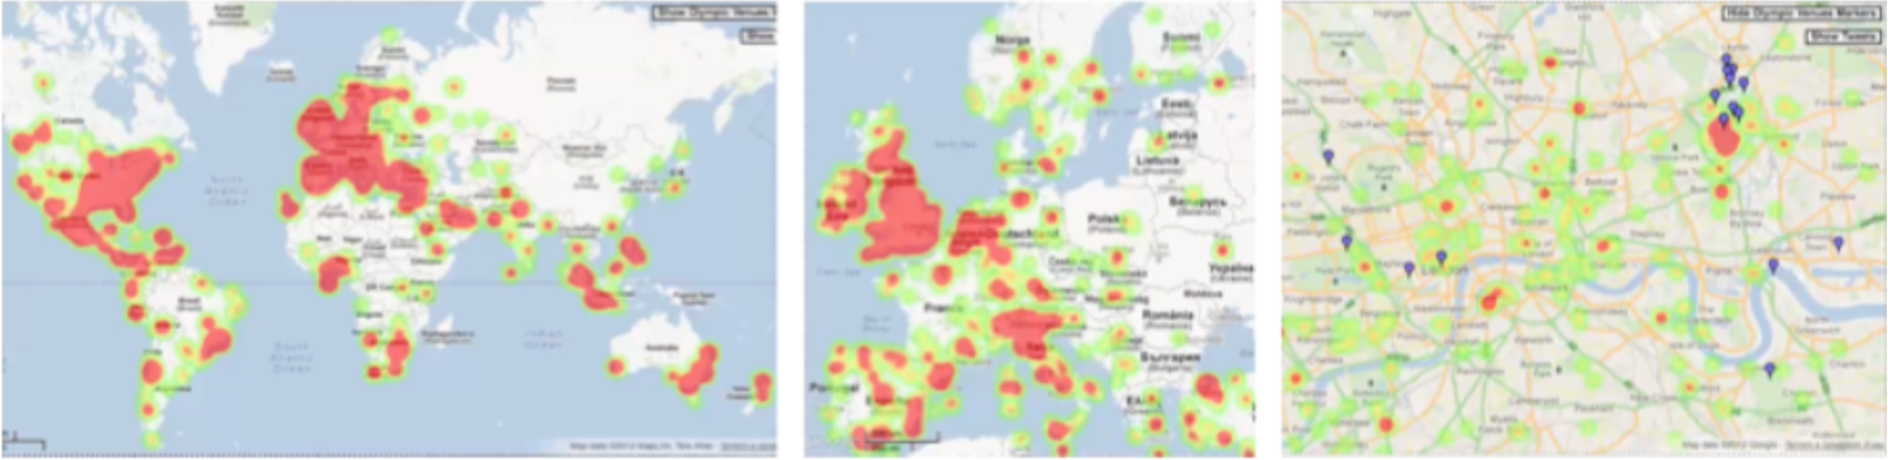
\includegraphics[width=0.8\textwidth]{img/london1}
} \\ 
\subfloat[]{
	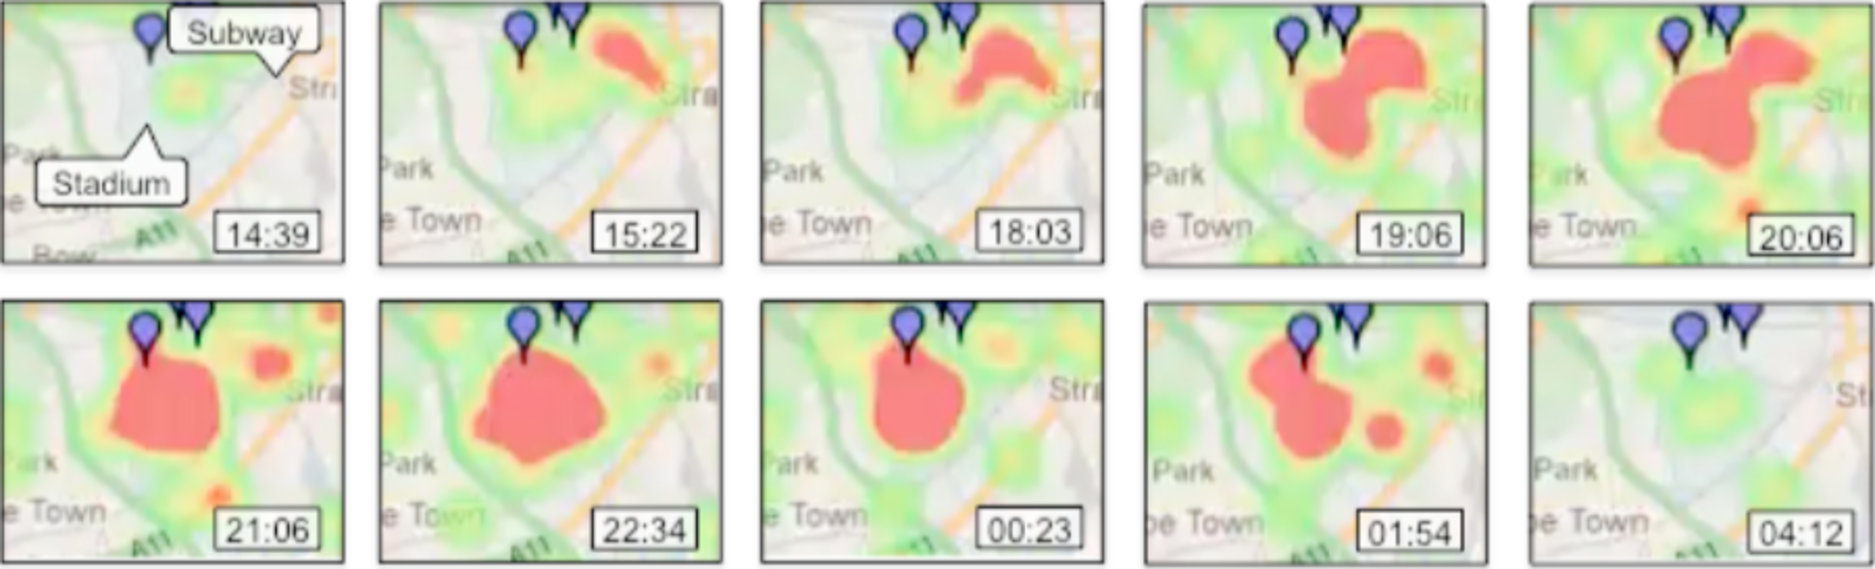
\includegraphics[width=0.8\textwidth]{img/london2}
}
\caption{The Figure (a) shows the people's interest at different zoom level during the Open ceremony of Olympic Games. Figure (b) shows the movement of the crowd in the surrounding of the Olympic Stadium at different time around the ceremony (source~\cite{DBLP:conf/semweb/BalduiniVDTPC13}).}
\label{fig:london-move}
\end{figure}

Figure~\ref{fig:london-move}(a) shows the attention of the people at different space granularity, i.e. World, Europe, City of London, during the London 2012 Open Ceremony. The information was extracted from Tweets selected exploiting keywords present in text of the content.
Figure~\ref{fig:london-move}(b) shows movements of the crowd before, during and after the Olympics open ceremony. Exploiting the Tweets position the system can clearly shows people arriving at the Olympic Stadium, entering the Olympic Stadium and leaving the Olympic Stadium.
Figure~\ref{fig:london-move}(a) and Figure~\ref{fig:london-move}(b) shows how the infrastructure can enable visual analytics. 
Both of the figure are based on the same data, but, while the former enables the observation of world-wide attention pattern, the latter offers insights of crowds' movements in a given area.

\subsection{Bottari} \label{sec:uda-bottari}
In 2011, an average of three million tweets per day was posted in Seoul and many of that carry the user's live opinion about restaurants, bars, cafes, and many other semi-public points of interest (POIs) in the city. 
The stream of data, which we continuously collected, results (i) incomplete, i.e. only 41\% of users rated at least the same POI, and (ii) inconsistent, i.e. many users rates a POI several times in different way.
BOTTARI~\cite{DBLP:journals/ws/BalduiniCDVHLKT12} exploits inductive and deductive stream reasoning (see Section \ref{sec:sr-rsp}) to continuously perform \textit{content}, \textit{spatial} and \textit{temporal} analysis on Social Media streams (i.e., Twitter) in order to understand how the Social Media users collectively perceive the POIs in a given area (e.g., Insadong's restaurants) and build a recommendation engine.

\begin{figure}[t]
	\centering
	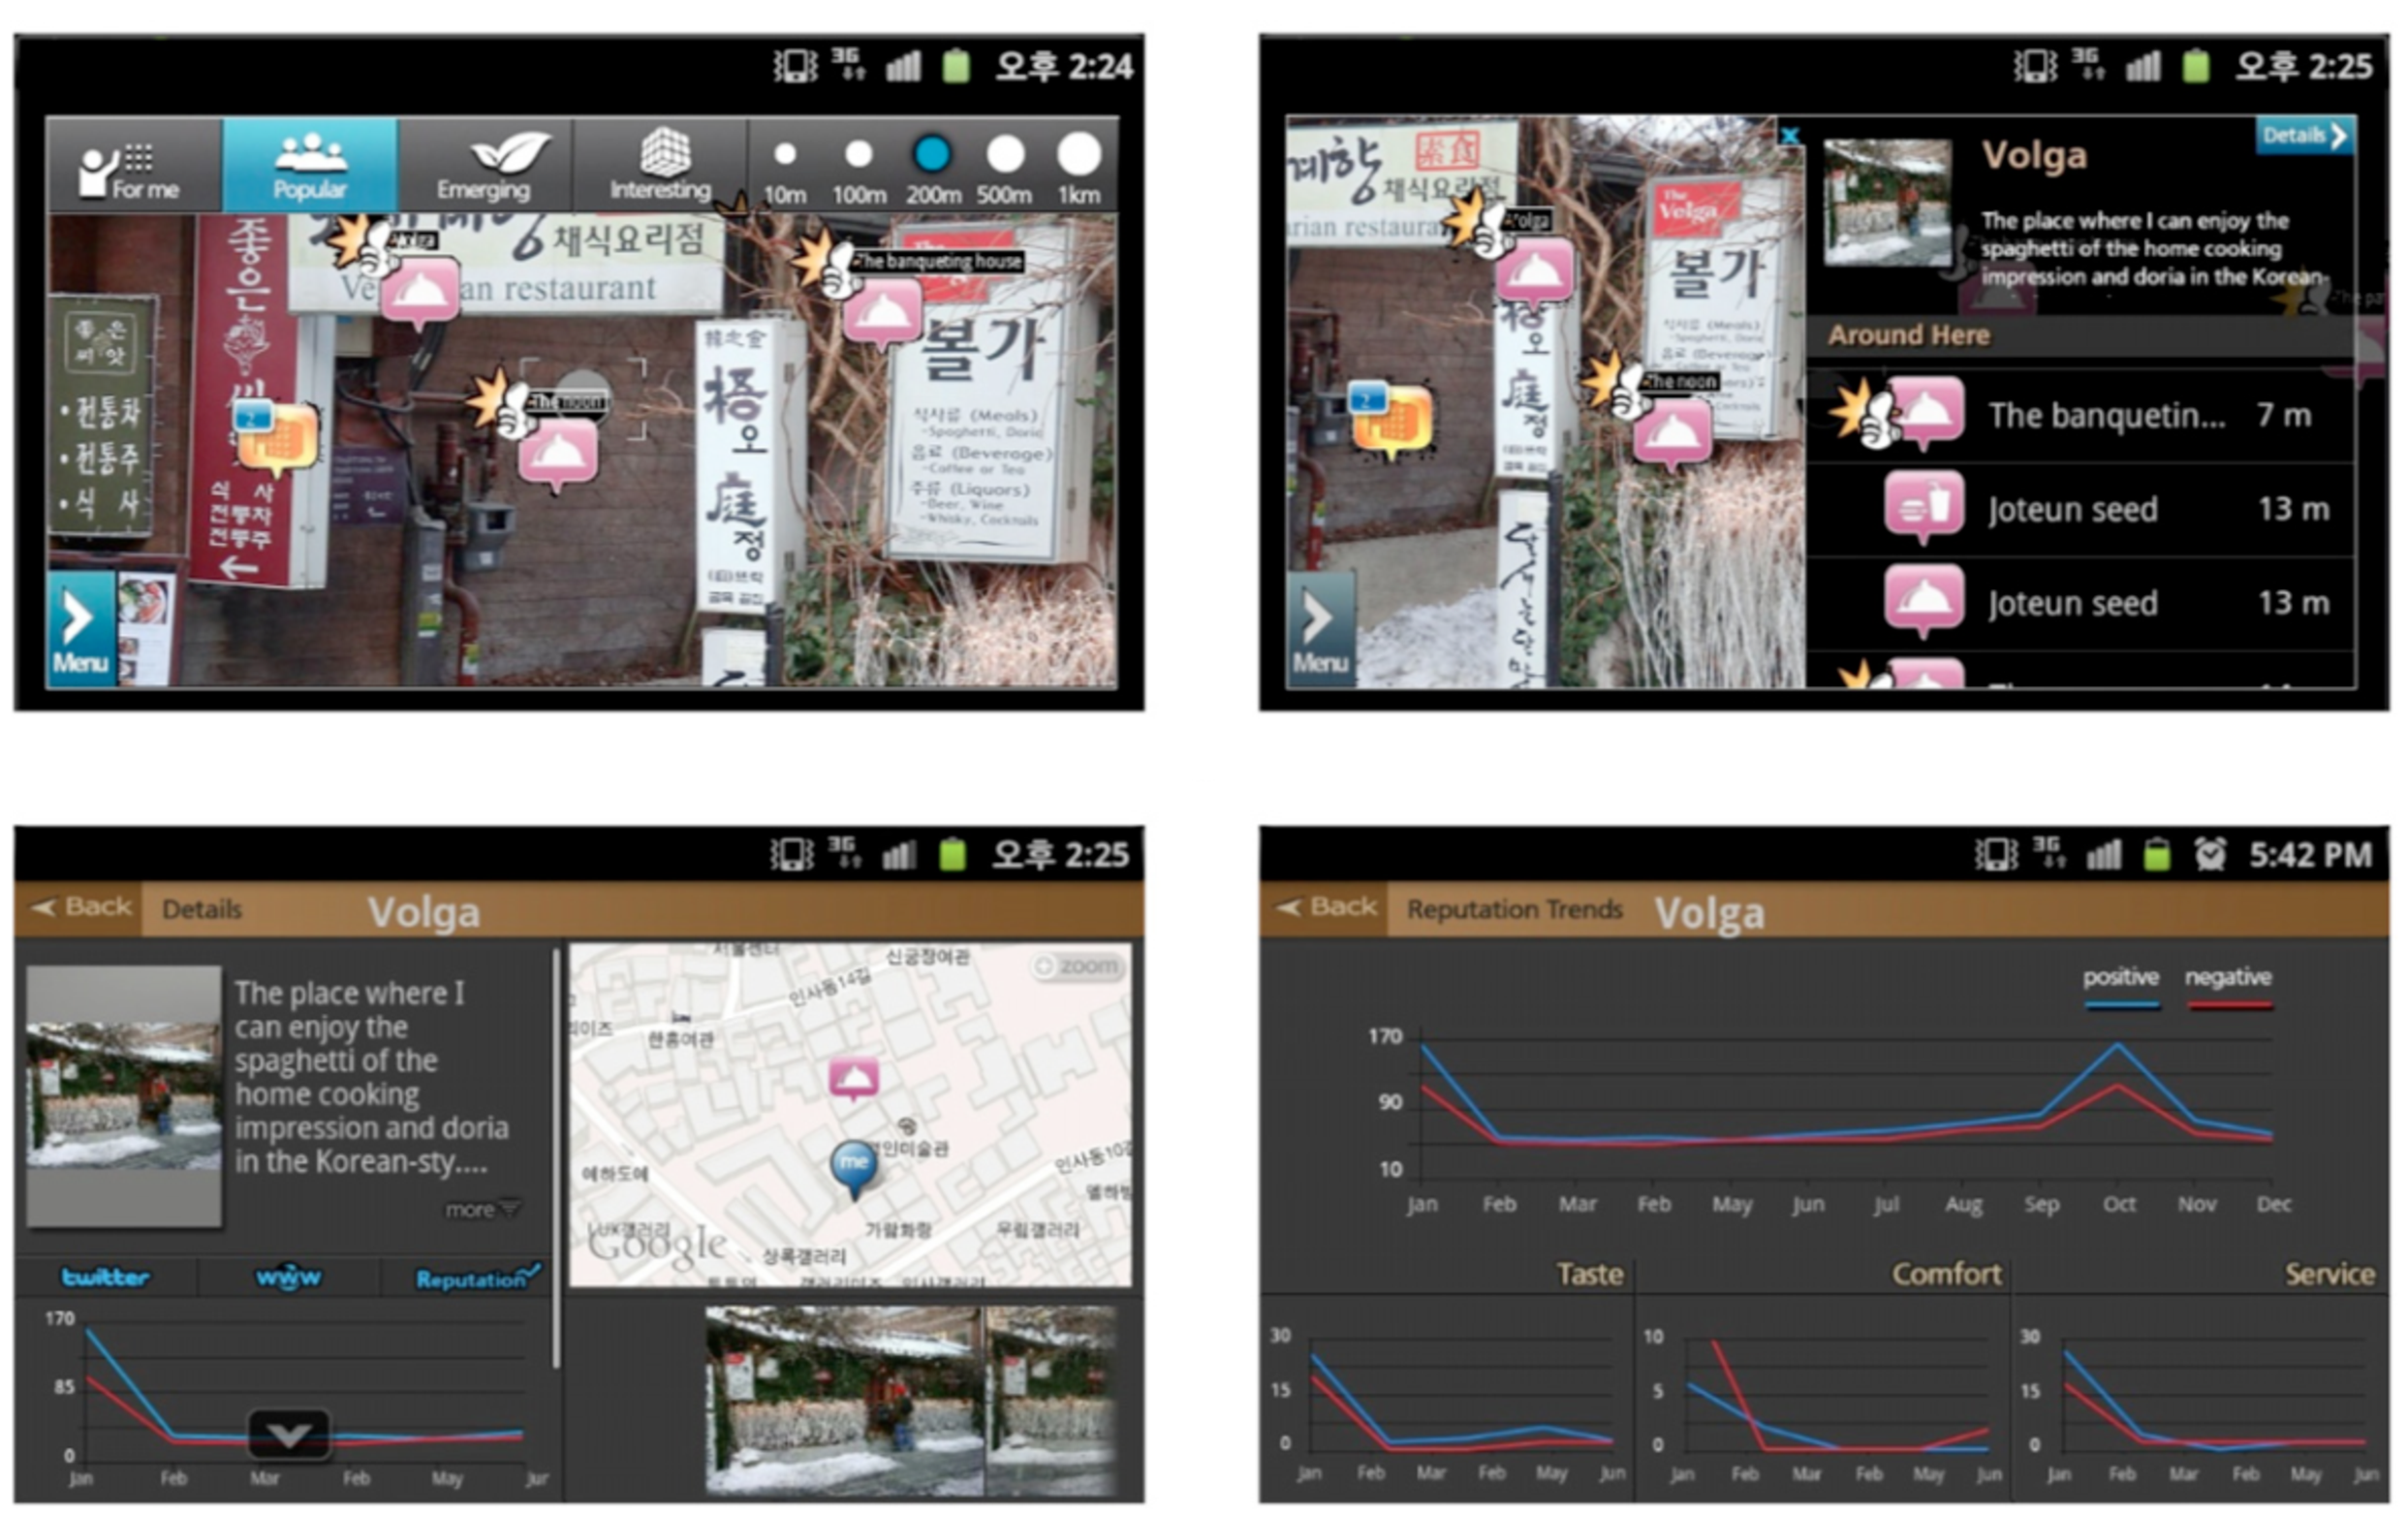
\includegraphics[width=0.75\textwidth]{img/bottari2.pdf}.
    \caption{BOTTARI visualizations (source~\cite{DBLP:conf/semweb/BalduiniVDTPC13}).}
    \label{fig:bottari-vis}
\end{figure}

BOTTARI is designed following an OBDI architecture (see Section \ref{sec:obdi-obda}). 
The infrastructure behind BOTTARI application is pluggable and is based on SLD framework (see Section \ref{sec:sld}). 
A first component in SLD pipeline casts in RDF the data item in the stream. 
A second downstream component performs the analysis exploiting the C-SPARQL Engine (see Section \ref{sec:vel-var-solutions}) as deductive stream reasoner
A last downstream component, based on the Statistical Unit Node Set (SUNS) \cite{tresp2009materializing,huang2010multivariate} approach, acts as inductive stream reasoner.
The data was continuously collected and modeled using BOTTARI ontology, an extension of SIOC vocabulary, to cope with the variety.

Figure~\ref{fig:bottari-vis} shows the various visualization offered by the augmented reality Android application that returns BOTTARI results to the end user. Such an application guides the user to the POI choice. The presented POIs are based on the deductive/inductive stream reasoning results and are personalized for the user.